% Options for packages loaded elsewhere
\PassOptionsToPackage{unicode}{hyperref}
\PassOptionsToPackage{hyphens}{url}
%
\documentclass[
]{article}
\usepackage{lmodern}
\usepackage{amssymb,amsmath}
\usepackage{ifxetex,ifluatex}
\ifnum 0\ifxetex 1\fi\ifluatex 1\fi=0 % if pdftex
  \usepackage[T1]{fontenc}
  \usepackage[utf8]{inputenc}
  \usepackage{textcomp} % provide euro and other symbols
\else % if luatex or xetex
  \usepackage{unicode-math}
  \defaultfontfeatures{Scale=MatchLowercase}
  \defaultfontfeatures[\rmfamily]{Ligatures=TeX,Scale=1}
\fi
% Use upquote if available, for straight quotes in verbatim environments
\IfFileExists{upquote.sty}{\usepackage{upquote}}{}
\IfFileExists{microtype.sty}{% use microtype if available
  \usepackage[]{microtype}
  \UseMicrotypeSet[protrusion]{basicmath} % disable protrusion for tt fonts
}{}
\makeatletter
\@ifundefined{KOMAClassName}{% if non-KOMA class
  \IfFileExists{parskip.sty}{%
    \usepackage{parskip}
  }{% else
    \setlength{\parindent}{0pt}
    \setlength{\parskip}{6pt plus 2pt minus 1pt}}
}{% if KOMA class
  \KOMAoptions{parskip=half}}
\makeatother
\usepackage{xcolor}
\IfFileExists{xurl.sty}{\usepackage{xurl}}{} % add URL line breaks if available
\IfFileExists{bookmark.sty}{\usepackage{bookmark}}{\usepackage{hyperref}}
\hypersetup{
  pdftitle={R Notebook},
  hidelinks,
  pdfcreator={LaTeX via pandoc}}
\urlstyle{same} % disable monospaced font for URLs
\usepackage[margin=1in]{geometry}
\usepackage{color}
\usepackage{fancyvrb}
\newcommand{\VerbBar}{|}
\newcommand{\VERB}{\Verb[commandchars=\\\{\}]}
\DefineVerbatimEnvironment{Highlighting}{Verbatim}{commandchars=\\\{\}}
% Add ',fontsize=\small' for more characters per line
\usepackage{framed}
\definecolor{shadecolor}{RGB}{248,248,248}
\newenvironment{Shaded}{\begin{snugshade}}{\end{snugshade}}
\newcommand{\AlertTok}[1]{\textcolor[rgb]{0.94,0.16,0.16}{#1}}
\newcommand{\AnnotationTok}[1]{\textcolor[rgb]{0.56,0.35,0.01}{\textbf{\textit{#1}}}}
\newcommand{\AttributeTok}[1]{\textcolor[rgb]{0.77,0.63,0.00}{#1}}
\newcommand{\BaseNTok}[1]{\textcolor[rgb]{0.00,0.00,0.81}{#1}}
\newcommand{\BuiltInTok}[1]{#1}
\newcommand{\CharTok}[1]{\textcolor[rgb]{0.31,0.60,0.02}{#1}}
\newcommand{\CommentTok}[1]{\textcolor[rgb]{0.56,0.35,0.01}{\textit{#1}}}
\newcommand{\CommentVarTok}[1]{\textcolor[rgb]{0.56,0.35,0.01}{\textbf{\textit{#1}}}}
\newcommand{\ConstantTok}[1]{\textcolor[rgb]{0.00,0.00,0.00}{#1}}
\newcommand{\ControlFlowTok}[1]{\textcolor[rgb]{0.13,0.29,0.53}{\textbf{#1}}}
\newcommand{\DataTypeTok}[1]{\textcolor[rgb]{0.13,0.29,0.53}{#1}}
\newcommand{\DecValTok}[1]{\textcolor[rgb]{0.00,0.00,0.81}{#1}}
\newcommand{\DocumentationTok}[1]{\textcolor[rgb]{0.56,0.35,0.01}{\textbf{\textit{#1}}}}
\newcommand{\ErrorTok}[1]{\textcolor[rgb]{0.64,0.00,0.00}{\textbf{#1}}}
\newcommand{\ExtensionTok}[1]{#1}
\newcommand{\FloatTok}[1]{\textcolor[rgb]{0.00,0.00,0.81}{#1}}
\newcommand{\FunctionTok}[1]{\textcolor[rgb]{0.00,0.00,0.00}{#1}}
\newcommand{\ImportTok}[1]{#1}
\newcommand{\InformationTok}[1]{\textcolor[rgb]{0.56,0.35,0.01}{\textbf{\textit{#1}}}}
\newcommand{\KeywordTok}[1]{\textcolor[rgb]{0.13,0.29,0.53}{\textbf{#1}}}
\newcommand{\NormalTok}[1]{#1}
\newcommand{\OperatorTok}[1]{\textcolor[rgb]{0.81,0.36,0.00}{\textbf{#1}}}
\newcommand{\OtherTok}[1]{\textcolor[rgb]{0.56,0.35,0.01}{#1}}
\newcommand{\PreprocessorTok}[1]{\textcolor[rgb]{0.56,0.35,0.01}{\textit{#1}}}
\newcommand{\RegionMarkerTok}[1]{#1}
\newcommand{\SpecialCharTok}[1]{\textcolor[rgb]{0.00,0.00,0.00}{#1}}
\newcommand{\SpecialStringTok}[1]{\textcolor[rgb]{0.31,0.60,0.02}{#1}}
\newcommand{\StringTok}[1]{\textcolor[rgb]{0.31,0.60,0.02}{#1}}
\newcommand{\VariableTok}[1]{\textcolor[rgb]{0.00,0.00,0.00}{#1}}
\newcommand{\VerbatimStringTok}[1]{\textcolor[rgb]{0.31,0.60,0.02}{#1}}
\newcommand{\WarningTok}[1]{\textcolor[rgb]{0.56,0.35,0.01}{\textbf{\textit{#1}}}}
\usepackage{graphicx}
\makeatletter
\def\maxwidth{\ifdim\Gin@nat@width>\linewidth\linewidth\else\Gin@nat@width\fi}
\def\maxheight{\ifdim\Gin@nat@height>\textheight\textheight\else\Gin@nat@height\fi}
\makeatother
% Scale images if necessary, so that they will not overflow the page
% margins by default, and it is still possible to overwrite the defaults
% using explicit options in \includegraphics[width, height, ...]{}
\setkeys{Gin}{width=\maxwidth,height=\maxheight,keepaspectratio}
% Set default figure placement to htbp
\makeatletter
\def\fps@figure{htbp}
\makeatother
\setlength{\emergencystretch}{3em} % prevent overfull lines
\providecommand{\tightlist}{%
  \setlength{\itemsep}{0pt}\setlength{\parskip}{0pt}}
\setcounter{secnumdepth}{5}
\newcommand{\R}{\textnormal{\sffamily\bfseries R}}
\def\code#1{\texttt{#1}}
\newtheorem{algorithm}{Algorithm}[section]
\usepackage{float}
\usepackage{booktabs}
\usepackage{longtable}
\usepackage{array}
\usepackage{multirow}
\usepackage{wrapfig}
\usepackage{colortbl}
\usepackage{pdflscape}
\usepackage{tabu}
\usepackage{threeparttable}
\usepackage{threeparttablex}
\usepackage[normalem]{ulem}
\usepackage{makecell}
\usepackage{xcolor}
\ifluatex
  \usepackage{selnolig}  % disable illegal ligatures
\fi

\title{R Notebook}
\author{}
\date{\vspace{-2.5em}}

\begin{document}
\maketitle

\textbf{Implementation}

In this section we present a practical illustration of the algorithms
discussed. For the sake of simplicity we use a random walk plus noise
model, i.e.~the most basic form of a linear Gaussian state-space model.
\begin{align}
y_{t}|x_{t} & \sim N(x_{t},\sigma^{2}) \\
x_{t}|x_{t-1} & \sim N(x_{t-1},\tau^{2}) \\
x_{0} & \sim N(m_{0},C_{0})
\end{align} As already mentioned before, in this case the filtering
distribution can be computed in closed form solutions using the Kalman
filter. However, this toy example will be used also to illustrate more
involved filtering strategies described in this work. We believe indeed
that it represents a useful starting point to understand the logic of
the algorithms which may be eventually replicated when dealing with more
complex models.\\
The filtering strategy is applied to 50 simulated data. Figure XX shows
the simulated true states sequence assuming as data generating process
the Equation (2) with \(\tau^{2}=1\) and simulated observed sequence
process form Equation (1) with \(\sigma^{2}=1\).

\begin{figure}[ht]

{\centering \includegraphics{draft-implementation-2_files/figure-latex/unnamed-chunk-3-1} 

}

\caption{Simulated random walk plus noise model}\label{fig:unnamed-chunk-3}
\end{figure}

The Kalman Filter for this model is implemented as described below.

\begin{algorithm} Kalman Filter for Random Walk plus Noise Model
\begin{itemize}
\item Initialize $\theta_{0} \sim N(m_{0},C_{0})$
\item For $t=1,...,n$:
\begin{enumerate}
\item Compute the one-step-ahead state predictive distribution at time $t-1$, notice that if $t=1$ no data have been observed yet and therefore $x_{1}|x_{0}\sim N(a_{1},R_{1})$ otherwise
\begin{align*}
x_{t}|y_{1:t-1} & \sim N(a_{t},R_{t})\\
a_{t} & = m_{t-1}\\
R_{t} & = C_{t-1}+\tau^2
\end{align*}
\item Compute the filtering distribution at time $t$ as $p(x_{t}|y_{1:t}) \propto p(x_{t}|y_{1:t-1})p(y_{t}|x_{t})$, i.e. the product of the one-step-ahead state predictive distribution and the likelihood
\begin{align*}
x_{t}|y_{1:t} & \sim N(m_{t},C_{t}) \\
m_{t} & = \big(1-\frac{R_{t}}{R_{t}+\sigma^2}\big)a_{t}+\frac{R_{t}}{R_{t}+\sigma^2}y_{t} \\
C_{t} & = \frac{R_{t}}{R_{t}+\sigma^2}\sigma^2
\end{align*}
\end{enumerate}
\end{itemize}
\end{algorithm}

Our \texttt{DLM} function implement in
\textnormal{\sffamily\bfseries R} replicate this steps.\\

\hrule
\hrule

\hfill\break
\texttt{DLM(data,sig2,tau2,m0,C0)}\\

\hrule

\textbf{Arguments}

\texttt{data} ~~the observed process. It has to be a vector or a
univariate time series.\\
\texttt{sig2} ~~the variance \(\sigma^{2}\) in Equation (1)\\
\texttt{tau2} ~~the variance \(\tau^{2}\) in Equation (2)\\
\texttt{m0} ~~central value of the normal prior state distribution\\
\texttt{C0} ~~variance of the normal prior state distribution

\hrule
\hrule

\begin{Shaded}
\begin{Highlighting}[]
\NormalTok{DLM}\OtherTok{\textless{}{-}}\ControlFlowTok{function}\NormalTok{(data,sig2,tau2,m0,C0)\{}
\NormalTok{  n  }\OtherTok{=} \FunctionTok{length}\NormalTok{(data)}
\NormalTok{  m  }\OtherTok{=} \FunctionTok{rep}\NormalTok{(}\DecValTok{0}\NormalTok{,n)}
\NormalTok{  C  }\OtherTok{=} \FunctionTok{rep}\NormalTok{(}\DecValTok{0}\NormalTok{,n)}
  \ControlFlowTok{for}\NormalTok{ (t }\ControlFlowTok{in} \DecValTok{1}\SpecialCharTok{:}\NormalTok{n)\{}
    \ControlFlowTok{if}\NormalTok{ (t}\SpecialCharTok{==}\DecValTok{1}\NormalTok{)\{}
\NormalTok{      a }\OtherTok{=}\NormalTok{ m0}
\NormalTok{      R }\OtherTok{=}\NormalTok{ C0 }\SpecialCharTok{+}\NormalTok{ tau2}
\NormalTok{    \}}\ControlFlowTok{else}\NormalTok{\{}
\NormalTok{      a }\OtherTok{=}\NormalTok{ m[t}\DecValTok{{-}1}\NormalTok{]}
\NormalTok{      R }\OtherTok{=}\NormalTok{ C[t}\DecValTok{{-}1}\NormalTok{] }\SpecialCharTok{+}\NormalTok{ tau2}
\NormalTok{    \}}
\NormalTok{    A }\OtherTok{=}\NormalTok{ R}\SpecialCharTok{/}\NormalTok{(R}\SpecialCharTok{+}\NormalTok{sig2)}
\NormalTok{    m[t] }\OtherTok{=}\NormalTok{ (}\DecValTok{1}\SpecialCharTok{{-}}\NormalTok{A)}\SpecialCharTok{*}\NormalTok{a }\SpecialCharTok{+}\NormalTok{ A}\SpecialCharTok{*}\NormalTok{y[t]}
\NormalTok{    C[t] }\OtherTok{=}\NormalTok{ A}\SpecialCharTok{*}\NormalTok{sig2}
\NormalTok{  \}}
  \FunctionTok{return}\NormalTok{(}\FunctionTok{list}\NormalTok{(}\AttributeTok{m=}\NormalTok{m,}\AttributeTok{C=}\NormalTok{C))}
\NormalTok{\}}
\end{Highlighting}
\end{Shaded}

In Figure XX below filtered states estimated using Kalman Filter with
\(x_{0} \sim N(0,100)\) and \(\sigma^{2}=\tau^{2}=1\) are compared to
the true states values. Notice how closely the filtered states follow
the observations and the goodness of the approximation of the true
states. 95 percent credible intervals are computed as
\[[E(\theta_{t}|y_{1:t})-z_{1-\alpha/2}\sqrt{V(\theta_{t}|y_{1:t})},E(\theta_{t}|y_{1:t})+z_{1-\alpha/2}\sqrt{V(\theta_{t}|y_{1:t})}]\]

\begin{figure}[ht]

{\centering 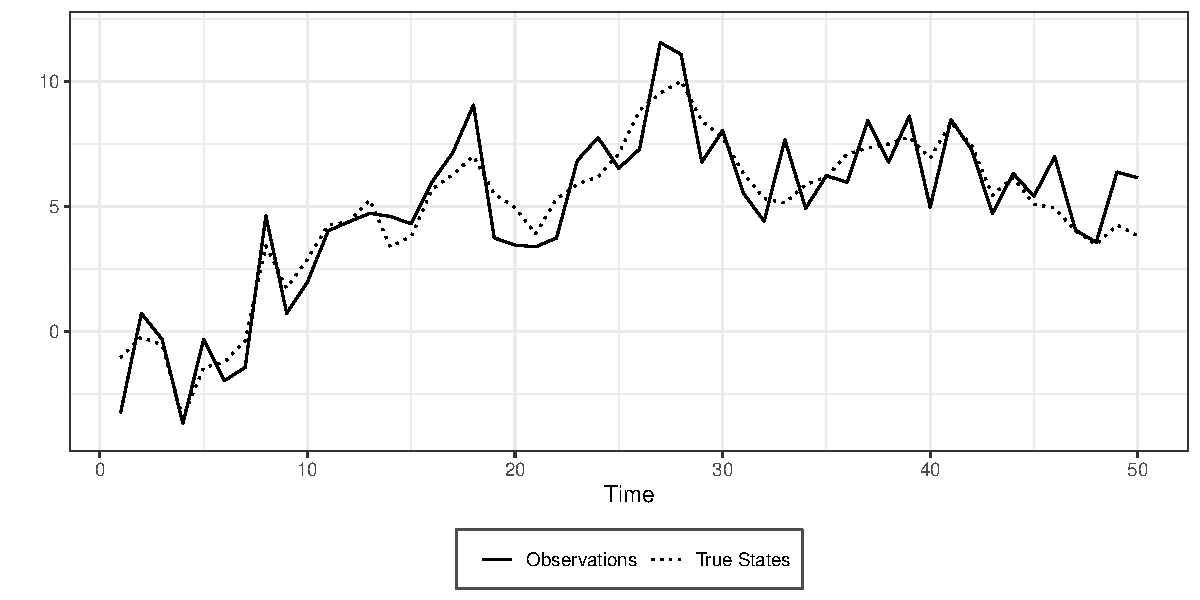
\includegraphics{draft-implementation-2_files/figure-latex/unnamed-chunk-5-1} 

}

\caption{Kalman Filtered States with credible interval (in red)}\label{fig:unnamed-chunk-5}
\end{figure}

The discussion of Kalman Filter will continue in Section XX where we
compare it to the Particle Filter.

\hfill\break

\section{Implementation}

Consider again the random walk plus noise model of section XX,the
challenge here is to estimate the filtered states using a Sequential
Importance Sampling algorithm. The main idea of the SIS applied to this
univariate linear gaussian model is described in the following
algorithm. We indicate with \(n\) the sample size of time observations
and with \(N\) the generated sample size for each step of the Sequenial
Monte Carlo.

\begin{algorithm} SIS filter for Random Walk plus Noise Model
\begin{itemize}
\item Let $\{(x_{0},w_{0})^{(i)}\}_{i=1}^{N}$ summarizes $p(x_{0}|y_{0})$ such that, for example, $E(g(x_{0})|y_{0}) \approx \sum_{i=1}^{N}w_{0}^{(i)}g(x_{0}^{(i)})$. In particular, initialize $(x_{0}^{(1)},...,x_{0}^{(N)})$ form $N(m_{0},C_{0})$ and set $w_{0}^{(i)}=N^{-1} \ \forall \ i=1,...,N$.
\item For $t=1,...,n$:
\begin{enumerate}
\item Draw $x_{t}^{(i)} \sim N(x_{t-1}^{(i)},\tau^2) \ \ i=1,...,N$ such that $\{(x_{t},w_{t-1})^{(i)}\}_{i=1}^{N}$ summarizes $p(x_{t}|y_{t-1})$
\item Set $w_{t}^{(i)} = w_{t-1}^{(i)}f_{N}(y_{t};x_{t}^{(i)},\sigma^2) \ \ i=1,...,N$ such that $\{(x_{t},w_{t})^{(i)}\}_{i=1}^{N}$ summarizes $p(x_{t}|y_{t})$
\item Set $p(x_{t}|y_{t})=\sum_{i=1}^{N}w_{t}^{(i)}\delta_{x_{t}^{(i)}}$
\end{enumerate}
\end{itemize}
\end{algorithm}

Our \texttt{SISfun} function implemented in
\textnormal{\sffamily\bfseries R} replicate this steps.\\

\hrule
\hrule

\hfill\break
\texttt{SISfun(data,N,m0,C0,tau,sigma)}\\

\hrule

\textbf{Arguments}

\texttt{data} ~~the observed process. It has to be a vector or a
univariate time series.\\
\texttt{N} ~~number of particles generated at each step\\
\texttt{m0} ~~central value of the normal prior state distribution\\
\texttt{C0} ~~variance of the normal prior state distribution\\
\texttt{tau} ~~the standard deviation \(\tau\) in Equation (2)\\
\texttt{sigma} ~~the standard deviation \(\sigma\) in Equation (1)

\hrule
\hrule

\begin{Shaded}
\begin{Highlighting}[]
\NormalTok{SISfun}\OtherTok{\textless{}{-}}\ControlFlowTok{function}\NormalTok{(data,N,m0,C0,tau,sigma)\{}
\NormalTok{  xs}\OtherTok{\textless{}{-}}\ConstantTok{NULL}
\NormalTok{  ws}\OtherTok{\textless{}{-}}\ConstantTok{NULL}
\NormalTok{  ess}\OtherTok{\textless{}{-}}\ConstantTok{NULL}
\NormalTok{  x  }\OtherTok{=} \FunctionTok{rnorm}\NormalTok{(N,m0,}\FunctionTok{sqrt}\NormalTok{(C0))}
\NormalTok{  w  }\OtherTok{=} \FunctionTok{rep}\NormalTok{(}\DecValTok{1}\SpecialCharTok{/}\NormalTok{N,N)}
  \ControlFlowTok{for}\NormalTok{(t }\ControlFlowTok{in} \DecValTok{1}\SpecialCharTok{:}\FunctionTok{length}\NormalTok{(data))\{}
\NormalTok{    x    }\OtherTok{=} \FunctionTok{rnorm}\NormalTok{(N,x,tau)                   }\CommentTok{\#sample from N(x\_\{t{-}1\},tau)}
\NormalTok{    w    }\OtherTok{=}\NormalTok{ w}\SpecialCharTok{*}\FunctionTok{dnorm}\NormalTok{(data[t],x,sigma)         }\CommentTok{\#update weight}
\NormalTok{    xs }\OtherTok{=} \FunctionTok{rbind}\NormalTok{(xs,x)}
\NormalTok{    ws }\OtherTok{=} \FunctionTok{rbind}\NormalTok{(ws,w)}
    
\NormalTok{    wnorm}\OtherTok{=}\NormalTok{ w}\SpecialCharTok{/}\FunctionTok{sum}\NormalTok{(w)                         }\CommentTok{\#normalized weight}
\NormalTok{    ESS  }\OtherTok{=} \DecValTok{1}\SpecialCharTok{/}\FunctionTok{sum}\NormalTok{(wnorm}\SpecialCharTok{\^{}}\DecValTok{2}\NormalTok{)                   }\CommentTok{\#effective sample size}
    
\NormalTok{    ess }\OtherTok{=}\FunctionTok{rbind}\NormalTok{(ess,ESS)}
\NormalTok{  \}}
  
  \FunctionTok{return}\NormalTok{(}\FunctionTok{list}\NormalTok{(}\AttributeTok{xs=}\NormalTok{xs,}\AttributeTok{ws=}\NormalTok{ws,}\AttributeTok{ess=}\NormalTok{ess))}
\NormalTok{\}}
\end{Highlighting}
\end{Shaded}

We have already discussed the reasons why the SIS algorithm does not
provide a good strategy in the filtering problem. We provide a graphical
intuition of what happens when we use such filtering strategy on a
simulated dataset. We decide to set \(N=1000\),\(m_{0}=0\),\(C_{0}=100\)
and \(\tau=\sigma=1\). The results shown in the following two plots
shows a clear degeneration of the effective sample size and bad fit of
filtered states with respect to the true values.

\begin{figure}[ht]

{\centering 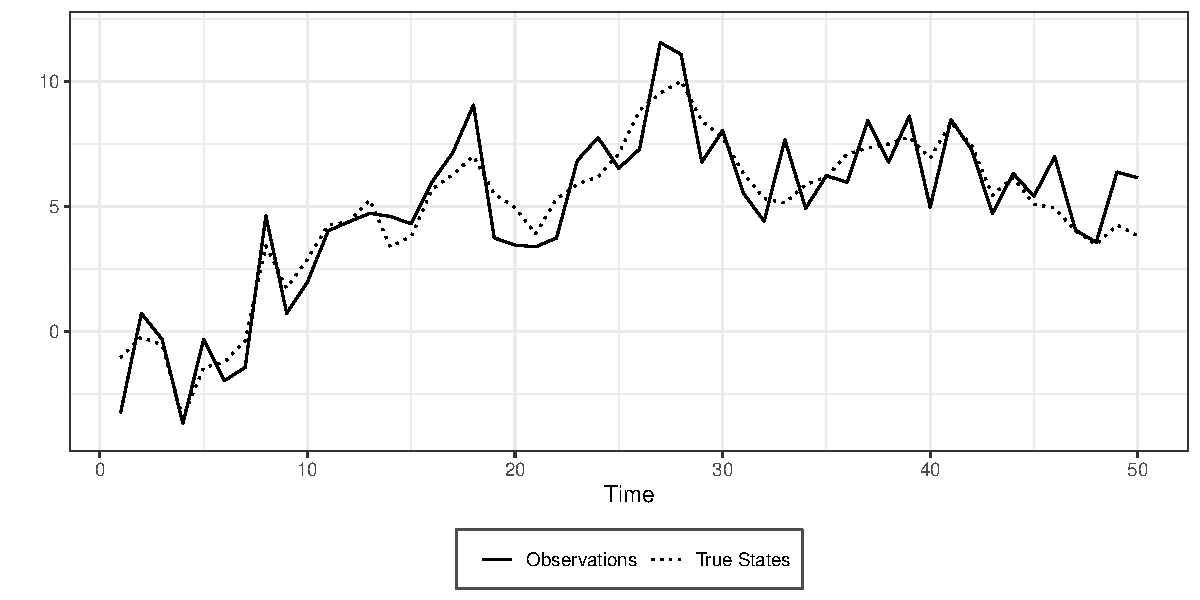
\includegraphics{draft-implementation-2_files/figure-latex/unnamed-chunk-8-1} 

}

\caption{a) SIS Filtered States with credible interval (in red). b) Effective sample size.}\label{fig:unnamed-chunk-8}
\end{figure}

\section{Implementation}

In this section, Bootstrap Particle Filter will be used to estimate
filtered states of the Random Walk plus Noise introduced in section XX.
The overall strategy replicate the SIS filter with the addition of a
ESS-based resampling step that applies when the effective sample size is
smaller than a predetermined threshold opportunely chosen (in our
example we decide to follow a common rule of thumb consisting in setting
the threshold at \(N/2\)). The steps are presented in the following
algorithm.

\begin{algorithm} BPF for Random Walk plus Noise Model
\begin{itemize}
\item Let $\{(x_{0},w_{0})^{(i)}\}_{i=1}^{N}$ summarizes $p(x_{0}|y_{0})$ such that, for example, $E(g(x_{0})|y_{0}) \approx \sum_{i=1}^{N}w_{0}^{(i)}g(x_{0}^{(i)})$. In particular, initialize $(x_{0}^{(1)},...,x_{0}^{(N)})$ form $N(m_{0},C_{0})$ and set $w_{0}^{(i)}=N^{-1} \ \forall \ i=1,...,N$.
\item For $t=1,...,n$:
\begin{enumerate}
\item Draw $x_{t}^{(i)} \sim N(x_{t-1}^{(i)},\tau^2) \ \ i=1,...,N$ such that $\{(x_{t},w_{t-1})^{(i)}\}_{i=1}^{N}$ summarizes $p(x_{t}|y_{t-1})$
\item Set $w_{t}^{(i)} = w_{t-1}^{(i)}f_{N}(y_{t};x_{t}^{(i)},\sigma^2) \ \ i=1,...,N$ such that $\{(x_{t},w_{t})^{(i)}\}_{i=1}^{N}$ summarizes $p(x_{t}|y_{t})$
\item if $ESS<N/2$ then
\begin{enumerate}
\item Draw a sample of size N, $(x_{t}^{(1)},...,x_{t}^{(N)})$, from the discrete distribution $P(x_{t}=x_{t}^{(i)})=w_{t}^{(i)},\ \ i=1,...,N$
\item Reset the weights: $w_{t}^{(i)}=N^{-1}$, $i=1,...,N$.
\end{enumerate}
\item Set $p(x_{t}|y_{t})=\sum_{i=1}^{N}w_{t}^{(i)}\delta_{x_{t}^{(i)}}$
\end{enumerate}
\end{itemize}
\end{algorithm}

These steps are resumed in our \texttt{PFfun} function.\\

\hrule
\hrule

\hfill\break
\texttt{PFfun(data,N,m0,C0,tau,sigma,r)}\\

\hrule

\textbf{Arguments}

\texttt{data} ~~the observed process. It has to be a vector or a
univariate time series.\\
\texttt{N} ~~number of particles generated at each step\\
\texttt{m0} ~~central value of the normal prior state distribution\\
\texttt{C0} ~~variance of the normal prior state distribution\\
\texttt{tau} ~~the standard deviation \(\tau\) in Equation (2)\\
\texttt{sigma} ~~the standard deviation \(\sigma\) in Equation (1)\\
\texttt{r} ~~ if present the threshold is set equal to \(N/r\)
otherwise, if missing, the threshold is set equal to \(N/2\)

\hrule
\hrule

\begin{Shaded}
\begin{Highlighting}[]
\NormalTok{PFfun}\OtherTok{\textless{}{-}}\ControlFlowTok{function}\NormalTok{(data,N,m0,C0,tau,sigma,r)\{}
  \ControlFlowTok{if}\NormalTok{(}\FunctionTok{missing}\NormalTok{(r))\{r}\OtherTok{=}\DecValTok{2}\NormalTok{\}}\ControlFlowTok{else}\NormalTok{\{\}}
\NormalTok{  xs}\OtherTok{\textless{}{-}}\ConstantTok{NULL}
\NormalTok{  ws}\OtherTok{\textless{}{-}}\ConstantTok{NULL}
\NormalTok{  ess}\OtherTok{\textless{}{-}}\ConstantTok{NULL}
\NormalTok{  x  }\OtherTok{=} \FunctionTok{rnorm}\NormalTok{(N,m0,}\FunctionTok{sqrt}\NormalTok{(C0))}
\NormalTok{  w  }\OtherTok{=} \FunctionTok{rep}\NormalTok{(}\DecValTok{1}\SpecialCharTok{/}\NormalTok{N,N)}
   
  \ControlFlowTok{for}\NormalTok{(t }\ControlFlowTok{in} \DecValTok{1}\SpecialCharTok{:}\FunctionTok{length}\NormalTok{(data))\{}
    
\NormalTok{    x}\OtherTok{\textless{}{-}}\FunctionTok{rnorm}\NormalTok{(N,x,tau)}
\NormalTok{    w1}\OtherTok{\textless{}{-}}\NormalTok{w}\SpecialCharTok{*}\FunctionTok{dnorm}\NormalTok{(data[t],x,sigma)}
    
\NormalTok{    w }\OtherTok{=}\NormalTok{ w1}\SpecialCharTok{/}\FunctionTok{sum}\NormalTok{(w1)}
\NormalTok{    ESS  }\OtherTok{=} \DecValTok{1}\SpecialCharTok{/}\FunctionTok{sum}\NormalTok{(w}\SpecialCharTok{\^{}}\DecValTok{2}\NormalTok{)}
    
    \ControlFlowTok{if}\NormalTok{(ESS}\SpecialCharTok{\textless{}}\NormalTok{(N}\SpecialCharTok{/}\NormalTok{r))\{}
\NormalTok{      index}\OtherTok{\textless{}{-}}\FunctionTok{sample}\NormalTok{(N,}\AttributeTok{size=}\NormalTok{N,}\AttributeTok{replace=}\NormalTok{T,}\AttributeTok{prob=}\NormalTok{w)}
\NormalTok{      x}\OtherTok{\textless{}{-}}\NormalTok{x[index]}
\NormalTok{      w}\OtherTok{\textless{}{-}}\FunctionTok{rep}\NormalTok{(}\DecValTok{1}\SpecialCharTok{/}\NormalTok{N,N)}
\NormalTok{    \}}\ControlFlowTok{else}\NormalTok{\{\}}
    
\NormalTok{    xs }\OtherTok{=} \FunctionTok{rbind}\NormalTok{(xs,x)}
\NormalTok{    ws }\OtherTok{=} \FunctionTok{rbind}\NormalTok{(ws,w)}
\NormalTok{    ess }\OtherTok{=}\FunctionTok{rbind}\NormalTok{(ess,ESS)}
\NormalTok{  \}}
  \FunctionTok{return}\NormalTok{(}\FunctionTok{list}\NormalTok{(}\AttributeTok{xs=}\NormalTok{xs,}\AttributeTok{ws=}\NormalTok{ws,}\AttributeTok{ess=}\NormalTok{ess))}
\NormalTok{\}}
\end{Highlighting}
\end{Shaded}

The estimated states of the Boostrap Particle Filter togheter with the
effective sample size are shown in Figure XX. We decide to set
\(N=1000\),\(m_{0}=0\),\(C_{0}=100\) and \(\tau=\sigma=1\). Notice how
the resampling step allows the effective sample size not to drop,
improving results.

\begin{figure}[ht]

{\centering 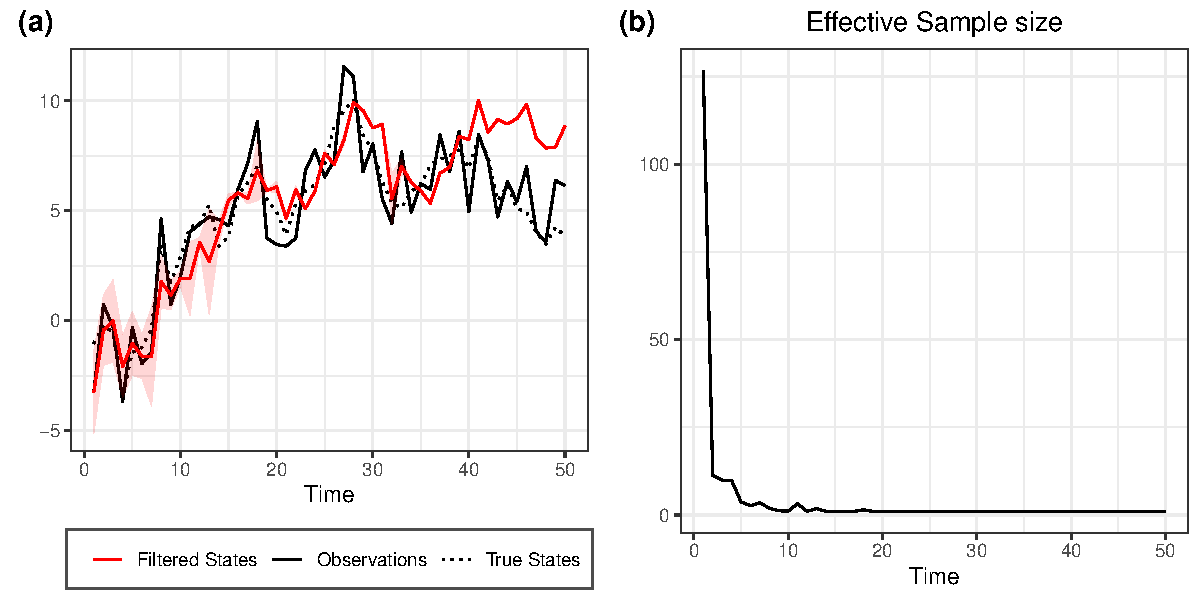
\includegraphics{draft-implementation-2_files/figure-latex/unnamed-chunk-11-1} 

}

\caption{a) PF Filtered States with credible interval (in red). b) Effective sample size (in black) with threshold (in yellow).}\label{fig:unnamed-chunk-11}
\end{figure}

Since the Random Walk plus Noise model allows for closed form solutions,
we want to compare the results of Boostrap Particle Filter(BPF) with
Kalman Filter(KF). As we can see from figure XX, when the number of
particles generated at any interaction increases the results for both
the estimated mean and the variance tend to converge {[}{[}SPIEGARE
PERCHE'{]}{]}. Moreover, comparing the Root Mean Square Errors of the
filtered states with respect to the true state values, when the sample
size increases the BPF decreases and, for large N, it reaches the
accuracy of the Kalman Filter.

\begin{longtable}[t]{cccc}
\caption{\label{tab:unnamed-chunk-13}Root Mean Square Errors}\\
\toprule
N & Threshold & KF & BPF\\
\midrule
100 & 0.5 & 0.879 & 0.888\\
1000 & 0.5 & 0.879 & 0.886\\
10000 & 0.5 & 0.879 & 0.878\\
\bottomrule
\end{longtable}

\begin{figure}[ht]

{\centering 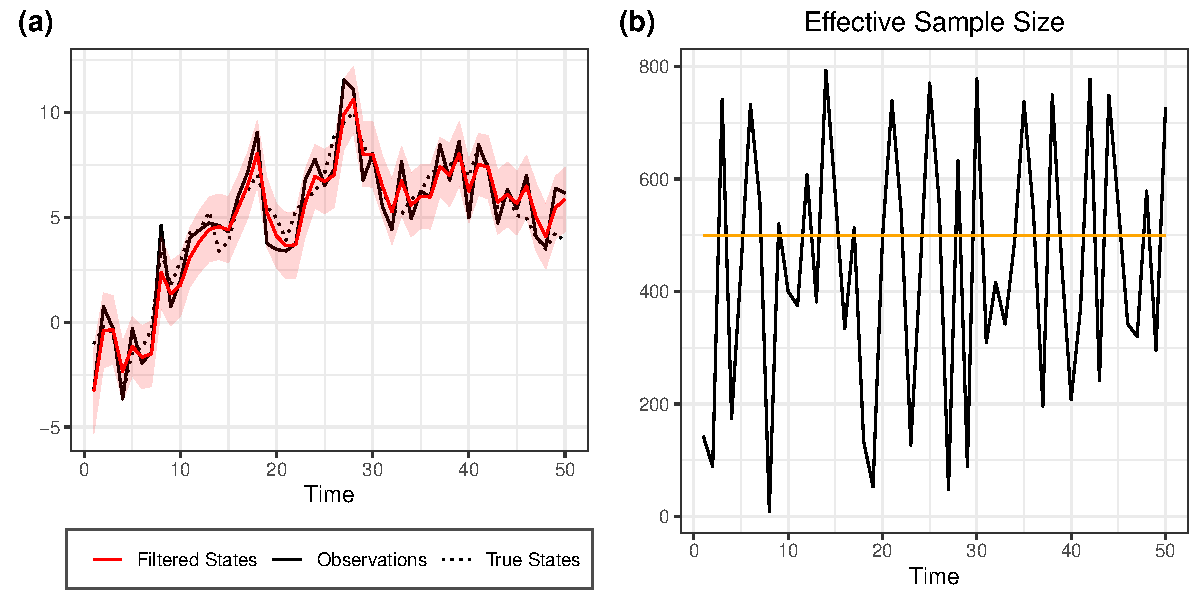
\includegraphics{draft-implementation-2_files/figure-latex/unnamed-chunk-14-1} 

}

\caption{Comparison Bootstrap Particle Filter(BPF) and Kalman Filter (KF) for increasing number of generated particles (N)}\label{fig:unnamed-chunk-14}
\end{figure}

\hfill\break

\section{Implementation}

\hfill\break
The Bootstrap Particle Filter Approach for the Random Walk plus Noise
Model described in Section XX can be improved accounting for the
observations in the importance transition density and it consists of
generating \(x_{t}\) from its conditional distribution given \(x_{t-1}\)
and \(y_{t}\). In the Normal model we are considering, the optimal
proposal will be a Normal density as well with mean and variance given
by \begin{align*}
\mu_{opt}=E(x_{t}|x_{t-1},y_{t})&=x_{t-1}+\frac{\tau^{2}}{\tau^{2}+\sigma^{2}}(y_{t}-x_{t-1})\\
\sigma_{opt}^{2}=V(x_{t}|x_{t-1},y_{t})&=\frac{\tau^{2}\sigma^{2}}{\tau^{2}+\sigma^{2}}
\end{align*} On the other hand, the incremental weights, using this
importance transition density, are proportional to the conditional
density of \(y_{t}\) given \(x_{t-1}=x_{t-1}^{(i)}\) , i.e
\(N(x_{t-1}^{(i)},\tau^{2}+\sigma^{2})\), evaluated at \(y_{t}\). In
other words the algorithm implemented in
\textnormal{\sffamily\bfseries R} is:

\begin{algorithm} GPF for Random Walk plus Noise Model
\begin{itemize}
\item Let $\{(x_{0},w_{0})^{(i)}\}_{i=1}^{N}$ summarizes $p(x_{0}|y_{0})$ such that, for example, $E(g(x_{0})|y_{0}) \approx \sum_{i=1}^{N}w_{0}^{(i)}g(x_{0}^{(i)})$. In particular, initialize $(x_{0}^{(1)},...,x_{0}^{(N)})$ from $N(m_{0},C_{0})$ and set $w_{0}^{(i)}=N^{-1} \ \forall \ i=1,...,N$.
\item Compute $\sigma_{opt}^{2}$ 
\item For $t=1,...,n$:
\begin{enumerate}
\item Compute $\mu_{opt}$
\item Draw $x_{t}^{(i)} \sim N(\mu_{opt},\sigma_{opt}^{2}) \ \ i=1,...,N$ such that $\{(x_{t},w_{t-1})^{(i)}\}_{i=1}^{N}$ summarizes $p(x_{t}|y_{t-1})$
\item Set $w_{t}^{(i)} = w_{t-1}^{(i)}f_{N}(y_{t};x_{t}^{(i)},\sigma^2+\tau^{2}) \ \ i=1,...,N$ such that $\{(x_{t},w_{t})^{(i)}\}_{i=1}^{N}$ summarizes $p(x_{t}|y_{t})$
\item if $ESS<N/2$ then
\begin{enumerate}
\item Draw a sample of size N, $(x_{t}^{(1)},...,x_{t}^{(N)})$, from the discrete distribution $P(x_{t}=x_{t}^{(i)})=w_{t}^{(i)},\ \ i=1,...,N$
\item Reset the weights: $w_{t}^{(i)}=N^{-1}$, $i=1,...,N$.
\end{enumerate}
\item Set $p(x_{t}|y_{t})=\sum_{i=1}^{N}w_{t}^{(i)}\delta_{x_{t}^{(i)}}$
\end{enumerate}
\end{itemize}
\end{algorithm}

The \texttt{GPFfun} function resume this passages.\\

\hrule
\hrule

\hfill\break
\texttt{GPFfun(data,N,m0,C0,tau,sigma,r)}\\

\hrule

\textbf{Arguments}

\texttt{data} ~~the observed process. It has to be a vector or a
univariate time series.\\
\texttt{N} ~~number of particles generated at each step\\
\texttt{m0} ~~central value of the normal prior state distribution\\
\texttt{C0} ~~variance of the normal prior state distribution\\
\texttt{tau} ~~the standard deviation \(\tau\) in Equation (2)\\
\texttt{sigma} ~~the standard deviation \(\sigma\) in Equation (1)\\
\texttt{r} ~~ if present the threshold is set equal to \(N/r\)
otherwise, if missing, the threshold is set equal to \(N/2\)

\hrule
\hrule

\begin{Shaded}
\begin{Highlighting}[]
\NormalTok{GPFfun}\OtherTok{\textless{}{-}}\ControlFlowTok{function}\NormalTok{(data,N,m0,C0,tau,sigma,r)\{}
  \ControlFlowTok{if}\NormalTok{(}\FunctionTok{missing}\NormalTok{(r))\{r}\OtherTok{=}\DecValTok{2}\NormalTok{\}}\ControlFlowTok{else}\NormalTok{\{\}}
\NormalTok{  xs}\OtherTok{\textless{}{-}}\ConstantTok{NULL}
\NormalTok{  ws}\OtherTok{\textless{}{-}}\ConstantTok{NULL}
\NormalTok{  ess}\OtherTok{\textless{}{-}}\ConstantTok{NULL}
\NormalTok{  x  }\OtherTok{=} \FunctionTok{rnorm}\NormalTok{(N,m0,}\FunctionTok{sqrt}\NormalTok{(C0))}
\NormalTok{  importancesd}\OtherTok{\textless{}{-}}\FunctionTok{sqrt}\NormalTok{(tau }\SpecialCharTok{{-}}\NormalTok{ tau}\SpecialCharTok{\^{}}\DecValTok{2} \SpecialCharTok{/}\NormalTok{(tau }\SpecialCharTok{+}\NormalTok{ sigma))}
\NormalTok{  predsd }\OtherTok{\textless{}{-}} \FunctionTok{sqrt}\NormalTok{(sigma}\SpecialCharTok{+}\NormalTok{tau)}
\NormalTok{  w  }\OtherTok{=} \FunctionTok{rep}\NormalTok{(}\DecValTok{1}\SpecialCharTok{/}\NormalTok{N,N)}
  
  \ControlFlowTok{for}\NormalTok{(t }\ControlFlowTok{in} \DecValTok{1}\SpecialCharTok{:}\FunctionTok{length}\NormalTok{(data))\{}
    
\NormalTok{    means}\OtherTok{\textless{}{-}}\NormalTok{x}\SpecialCharTok{+}\NormalTok{(tau}\SpecialCharTok{/}\NormalTok{(tau}\SpecialCharTok{+}\NormalTok{sigma))}\SpecialCharTok{*}\NormalTok{(data[t]}\SpecialCharTok{{-}}\NormalTok{x)}
\NormalTok{    x}\OtherTok{\textless{}{-}}\FunctionTok{rnorm}\NormalTok{(N,means,importancesd)}
\NormalTok{    w1}\OtherTok{\textless{}{-}}\NormalTok{w}\SpecialCharTok{*}\FunctionTok{dnorm}\NormalTok{(data[t],x,predsd)}
    
\NormalTok{    w }\OtherTok{=}\NormalTok{ w1}\SpecialCharTok{/}\FunctionTok{sum}\NormalTok{(w1)}
\NormalTok{    ESS  }\OtherTok{=} \DecValTok{1}\SpecialCharTok{/}\FunctionTok{sum}\NormalTok{(w}\SpecialCharTok{\^{}}\DecValTok{2}\NormalTok{)}
    
    \ControlFlowTok{if}\NormalTok{(ESS}\SpecialCharTok{\textless{}}\NormalTok{(N}\SpecialCharTok{/}\NormalTok{r))\{}
\NormalTok{      index}\OtherTok{\textless{}{-}}\FunctionTok{sample}\NormalTok{(N,}\AttributeTok{size=}\NormalTok{N,}\AttributeTok{replace=}\NormalTok{T,}\AttributeTok{prob=}\NormalTok{w)}
\NormalTok{      x}\OtherTok{\textless{}{-}}\NormalTok{x[index]}
\NormalTok{      w}\OtherTok{\textless{}{-}}\FunctionTok{rep}\NormalTok{(}\DecValTok{1}\SpecialCharTok{/}\NormalTok{N,N)}
\NormalTok{    \}}\ControlFlowTok{else}\NormalTok{\{\}}
    
\NormalTok{    xs }\OtherTok{=} \FunctionTok{rbind}\NormalTok{(xs,x)}
\NormalTok{    ws }\OtherTok{=} \FunctionTok{rbind}\NormalTok{(ws,w)}
\NormalTok{    ess }\OtherTok{=}\FunctionTok{rbind}\NormalTok{(ess,ESS)}
\NormalTok{  \}}
  \FunctionTok{return}\NormalTok{(}\FunctionTok{list}\NormalTok{(}\AttributeTok{xs=}\NormalTok{xs,}\AttributeTok{ws=}\NormalTok{ws,}\AttributeTok{ess=}\NormalTok{ess))}
\NormalTok{\}}
\end{Highlighting}
\end{Shaded}

\begin{figure}[ht]

{\centering 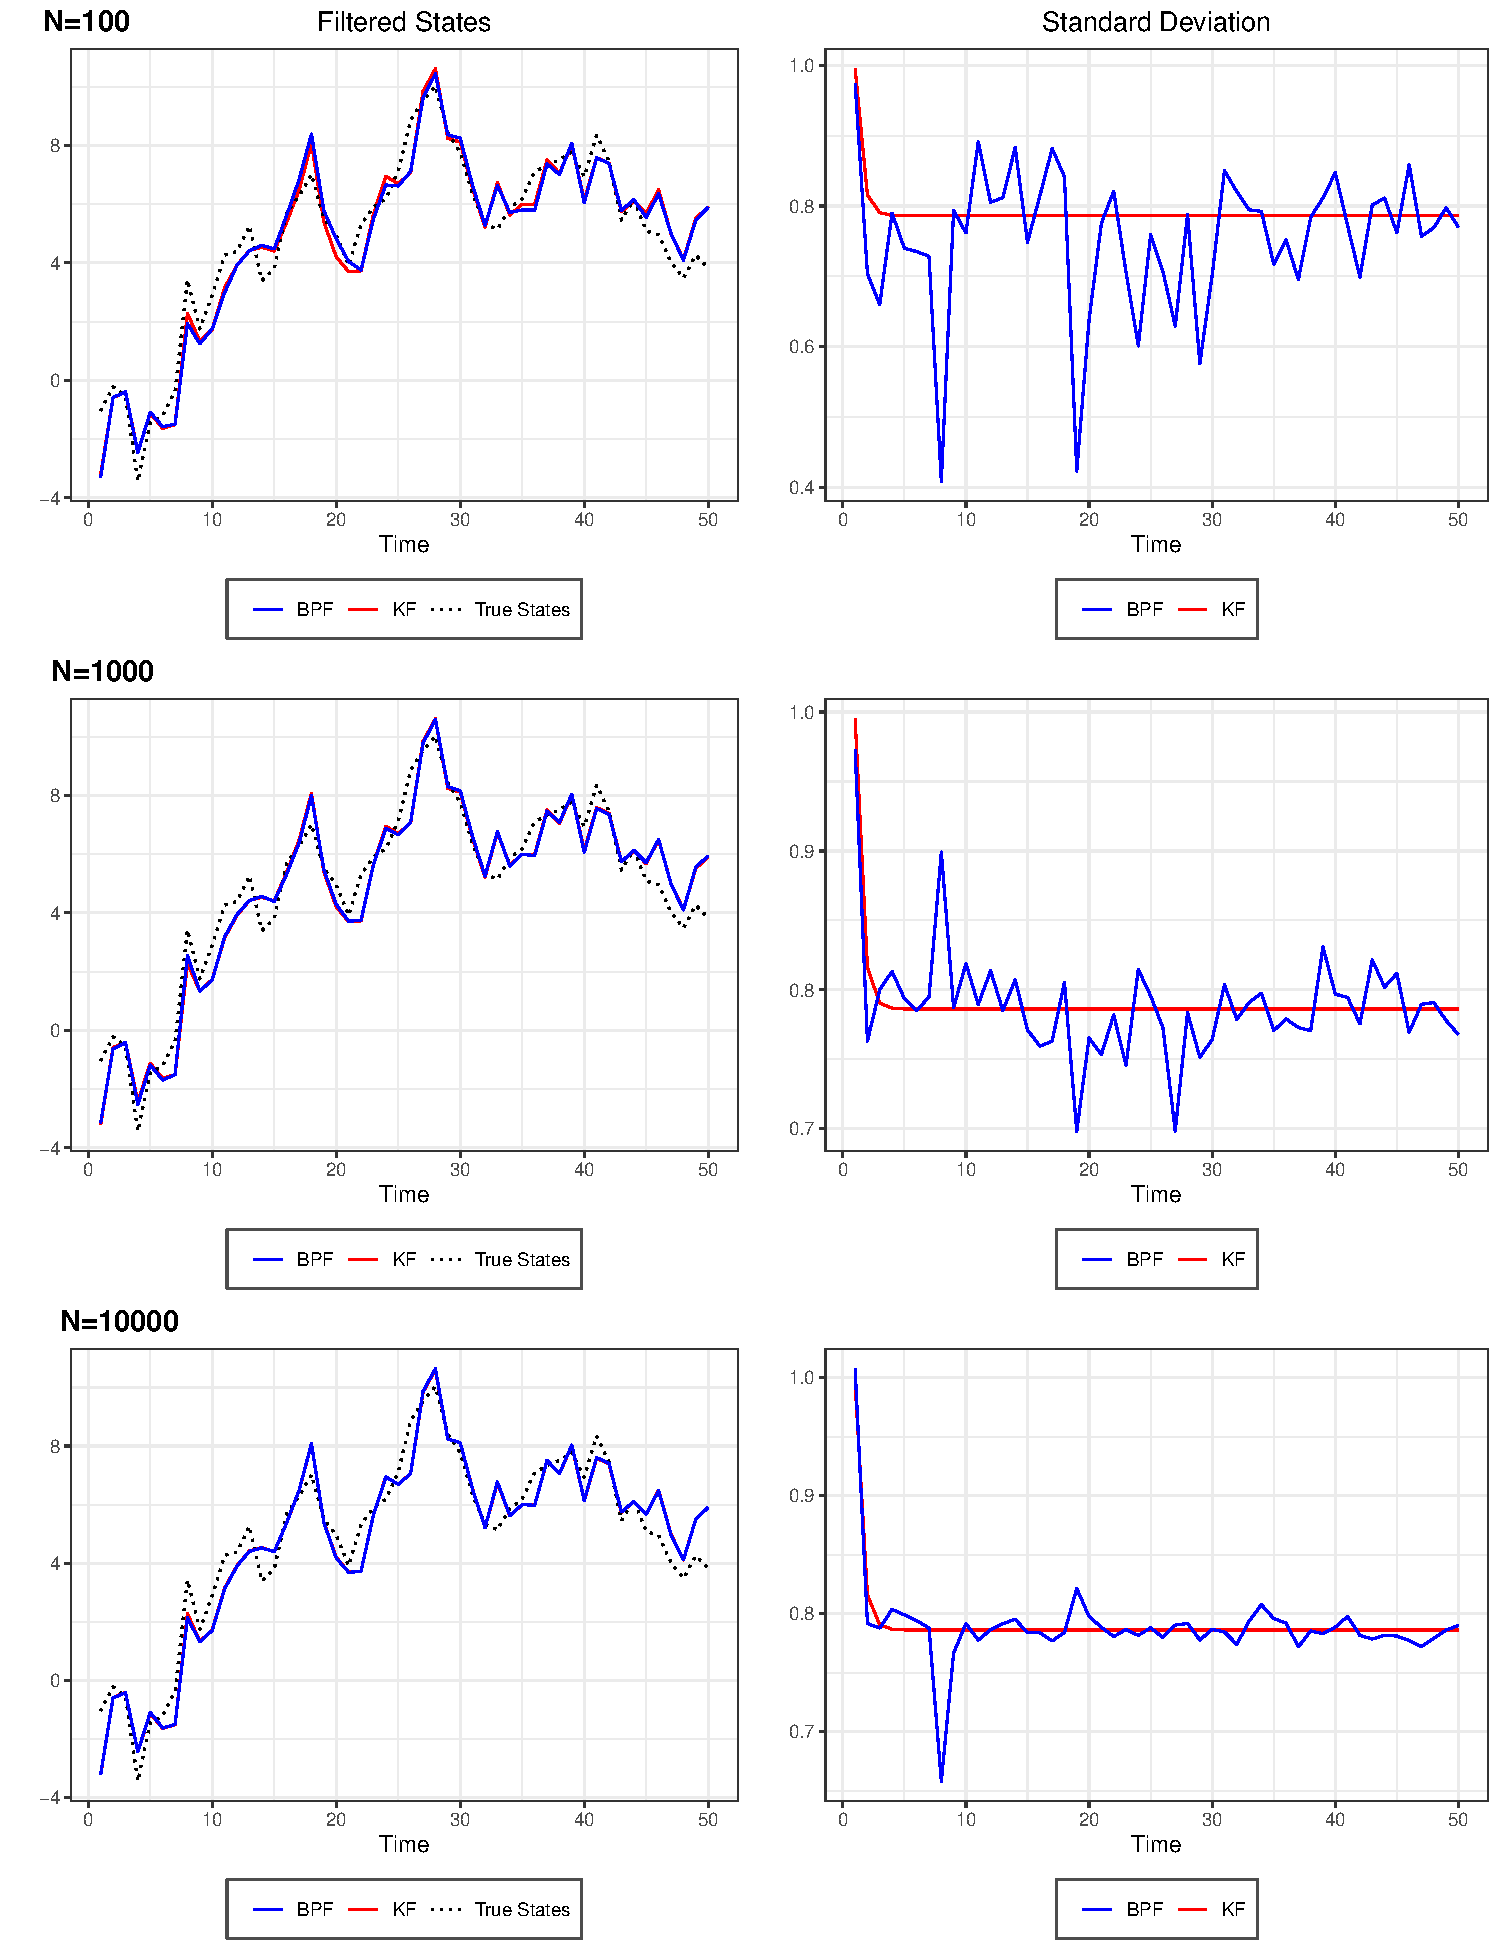
\includegraphics{draft-implementation-2_files/figure-latex/unnamed-chunk-17-1} 

}

\caption{a) GPF Filtered States with credible interval (in red). b) Effective sample size (in black) with threshold (in yellow).}\label{fig:unnamed-chunk-17}
\end{figure}

Let's provide directly a brief comparison between the Bootstrap Particle
Filter (BPF) and the Guided Particle Filter (GPF). As we can see from
the Figure XX, the Guided Particle Filter provides point estimates that
are slightly better with respect to the ones of the BPF, and this is
confirmed by the Table showing the RMSE. Moreover, also the variance is
better, suggesting for higher precision.

\begin{longtable}[t]{cccc}
\caption{\label{tab:unnamed-chunk-19}Root Mean Square Errors}\\
\toprule
N & Threshold & BPF & GPF\\
\midrule
1000 & 0.50 & 0.916 & 0.880\\
1000 & 0.25 & 0.895 & 0.862\\
1000 & 0.10 & 0.869 & 0.881\\
\bottomrule
\end{longtable}

\begin{figure}[ht]

{\centering 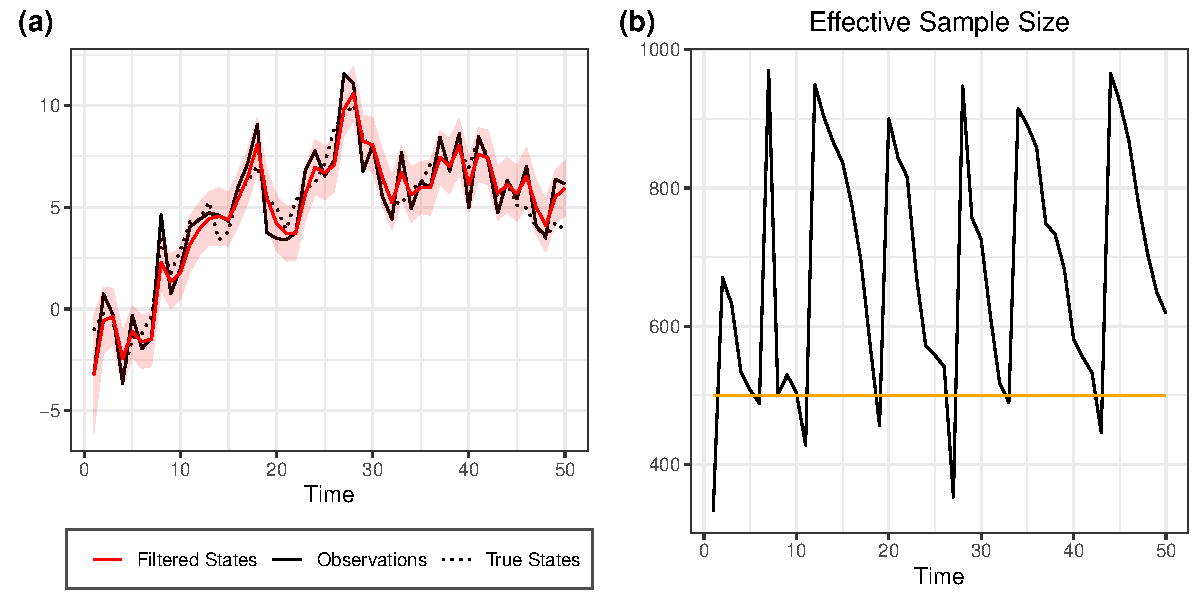
\includegraphics{draft-implementation-2_files/figure-latex/unnamed-chunk-20-1} 

}

\caption{Comparison Bootstrap Particle Filter(BPF) and Guided Particle Filter (GPF), number of generated particles N=1000}\label{fig:unnamed-chunk-20}
\end{figure}

\textbf{Implementation}

For illustration purposes, we are going implement an auxiliary particle
filter with auxiliary function \(g(x_{t-1})=E(x_{t}|x_{t-1})=x_{t-1}\).

\begin{algorithm} APF for Random Walk plus Noise Model
\begin{itemize}
\item Let $\{(x_{0},w_{0})^{(i)}\}_{i=1}^{N}$ summarizes $p(x_{0}|y_{0})$ such that, for example, $E(g(x_{0})|y_{0}) \approx \sum_{i=1}^{N}w_{0}^{(i)}g(x_{0}^{(i)})$. In particular, initialize $(x_{0}^{(1)},...,x_{0}^{(N)})$ from $N(m_{0},C_{0})$ and set $w_{0}^{(i)}=N^{-1} \ \forall \ i=1,...,N$.
\item For $t=1,...,n$:
\begin{enumerate}
\item For $k=1,...,N$:
\begin{enumerate}
\item Draw $I_{k}$ with $P(I_{k}) \propto w_{t-1}^{(i)}f(y_{t}|g(x_{t-1}^{(i)})) $
\item Draw $x_{t}^{(k)} \sim N(x_{t-1}^{(I_{k})},\tau^2)$
\item Set  $\tilde{w}_{t}^{(k)} = \frac{f_{N}(y_{t}|x_{t}^{(k)})}{f_{N}(y_{t}|g(x_{t-1}^{(I_{k})}))}$
\end{enumerate}
\item Normalize the weights: $w_{t}^{(i)}=\frac{\tilde{w}_{t}^{(i)}}{\sum_{j=1}^{N}(\tilde{w}_{t}^{(j)})}$
\item Compute $ESS=\Bigg(\sum_{i=1}^{N}(w_{t}^{(i)})^{2}\Bigg)^{-1}$
\item if $ESS<N/2$ then
\begin{enumerate}
\item Draw a sample of size N, $(x_{t}^{(1)},...,x_{t}^{(N)})$, from the discrete distribution $P(x_{t}=x_{t}^{(i)})=w_{t}^{(i)},\ \ i=1,...,N$
\item Reset the weights: $w_{t}^{(i)}=N^{-1}$, $i=1,...,N$.
\end{enumerate}
\item Set $p(x_{t}|y_{1:t})=\sum_{i=1}^{N}w_{t}^{(i)}\delta_{x_{t}^{(i)}}$
\end{enumerate}
\end{itemize}
\end{algorithm}

The \texttt{APFfun} function resume this passages.\\

\hrule
\hrule

\hfill\break
\texttt{APFfun(data,N,m0,C0,tau,sigma,r)}\\

\hrule

\textbf{Arguments}

\texttt{data} ~~the observed process. It has to be a vector or a
univariate time series.\\
\texttt{N} ~~number of particles generated at each step\\
\texttt{m0} ~~central value of the normal prior state distribution\\
\texttt{C0} ~~variance of the normal prior state distribution\\
\texttt{tau} ~~the standard deviation \(\tau\) in Equation (2)\\
\texttt{sigma} ~~the standard deviation \(\sigma\) in Equation (1)\\
\texttt{r} ~~ if present the threshold is set equal to \(N/r\)
otherwise, if missing, the threshold is set equal to \(N/2\)

\hrule
\hrule

\begin{Shaded}
\begin{Highlighting}[]
\NormalTok{APFfun}\OtherTok{\textless{}{-}}\ControlFlowTok{function}\NormalTok{(data,N,m0,C0,tau,sigma,r)\{}
  \ControlFlowTok{if}\NormalTok{(}\FunctionTok{missing}\NormalTok{(r))\{r}\OtherTok{=}\DecValTok{2}\NormalTok{\}}\ControlFlowTok{else}\NormalTok{\{\}}
\NormalTok{  xs}\OtherTok{\textless{}{-}}\ConstantTok{NULL}
\NormalTok{  ws}\OtherTok{\textless{}{-}}\ConstantTok{NULL}
\NormalTok{  ess}\OtherTok{\textless{}{-}}\ConstantTok{NULL}
\NormalTok{  x  }\OtherTok{=} \FunctionTok{rnorm}\NormalTok{(N,m0,}\FunctionTok{sqrt}\NormalTok{(C0))}
\NormalTok{  w  }\OtherTok{=} \FunctionTok{rep}\NormalTok{(}\DecValTok{1}\SpecialCharTok{/}\NormalTok{N,N)}
  
  \ControlFlowTok{for}\NormalTok{(t }\ControlFlowTok{in} \DecValTok{1}\SpecialCharTok{:}\FunctionTok{length}\NormalTok{(data))\{}
    
\NormalTok{    weight }\OtherTok{=}\NormalTok{ w}\SpecialCharTok{*}\FunctionTok{dnorm}\NormalTok{(data[t],x,sigma)}
\NormalTok{    k   }\OtherTok{=} \FunctionTok{sample}\NormalTok{(}\DecValTok{1}\SpecialCharTok{:}\NormalTok{N,}\AttributeTok{size=}\NormalTok{N,}\AttributeTok{replace=}\ConstantTok{TRUE}\NormalTok{,}\AttributeTok{prob=}\NormalTok{weight)}
\NormalTok{    x1   }\OtherTok{=} \FunctionTok{rnorm}\NormalTok{(N,x[k],tau)}
\NormalTok{    lw  }\OtherTok{=} \FunctionTok{dnorm}\NormalTok{(data[t],x1,sigma,}\AttributeTok{log=}\ConstantTok{TRUE}\NormalTok{)}\SpecialCharTok{{-}}\FunctionTok{dnorm}\NormalTok{(data[t],x[k],sigma,}\AttributeTok{log=}\ConstantTok{TRUE}\NormalTok{)}
\NormalTok{    w   }\OtherTok{=} \FunctionTok{exp}\NormalTok{(lw)}
\NormalTok{    w   }\OtherTok{=}\NormalTok{ w}\SpecialCharTok{/}\FunctionTok{sum}\NormalTok{(w)}
\NormalTok{    ESS  }\OtherTok{=} \DecValTok{1}\SpecialCharTok{/}\FunctionTok{sum}\NormalTok{(w}\SpecialCharTok{\^{}}\DecValTok{2}\NormalTok{)}
    
    \ControlFlowTok{if}\NormalTok{(ESS}\SpecialCharTok{\textless{}}\NormalTok{(N}\SpecialCharTok{/}\NormalTok{r))\{}
\NormalTok{      index}\OtherTok{\textless{}{-}}\FunctionTok{sample}\NormalTok{(N,}\AttributeTok{size=}\NormalTok{N,}\AttributeTok{replace=}\NormalTok{T,}\AttributeTok{prob=}\NormalTok{w)}
\NormalTok{      x1}\OtherTok{\textless{}{-}}\NormalTok{x1[index]}
\NormalTok{      w}\OtherTok{\textless{}{-}}\FunctionTok{rep}\NormalTok{(}\DecValTok{1}\SpecialCharTok{/}\NormalTok{N,N)}
\NormalTok{    \}}\ControlFlowTok{else}\NormalTok{\{\}}
    
\NormalTok{    x }\OtherTok{\textless{}{-}}\NormalTok{ x1}
\NormalTok{    xs }\OtherTok{=} \FunctionTok{rbind}\NormalTok{(xs,x)}
\NormalTok{    ws }\OtherTok{=} \FunctionTok{rbind}\NormalTok{(ws,w)}
\NormalTok{    ess }\OtherTok{=}\FunctionTok{rbind}\NormalTok{(ess,ESS)}
    
\NormalTok{  \}}
  \FunctionTok{return}\NormalTok{(}\FunctionTok{list}\NormalTok{(}\AttributeTok{xs=}\NormalTok{xs,}\AttributeTok{ws=}\NormalTok{ws,}\AttributeTok{ess=}\NormalTok{ess))}
\NormalTok{\}}
\end{Highlighting}
\end{Shaded}

\begin{figure}[ht]

{\centering 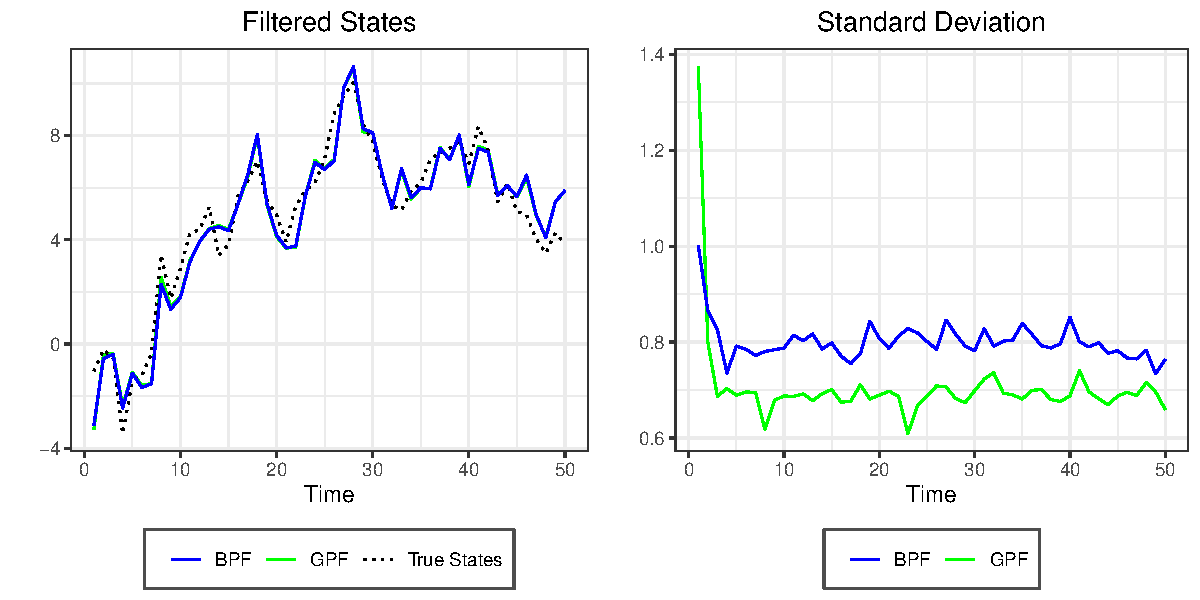
\includegraphics{draft-implementation-2_files/figure-latex/unnamed-chunk-23-1} 

}

\caption{a) APF Filtered States with credible interval (in red). b) Effective sample size (in black) with threshold (in yellow).}\label{fig:unnamed-chunk-23}
\end{figure}

Let's compare the Auxiliary Particle Filter (APF) and the Bootstrap
Particle Filter (BPF).

\begin{figure}[ht]

{\centering \includegraphics{draft-implementation-2_files/figure-latex/unnamed-chunk-24-1} 

}

\caption{Comparison Bootstrap Particle Filter(BPF) and Guided Particle Filter (GPF), number of generated particles N=1000}\label{fig:unnamed-chunk-24}
\end{figure}

\begin{longtable}[t]{cccc}
\caption{\label{tab:unnamed-chunk-26}Root Mean Square Errors}\\
\toprule
N & Threshold & BPF & APF\\
\midrule
1000 & 0.50 & 0.885 & 0.875\\
1000 & 0.25 & 0.893 & 0.892\\
1000 & 0.10 & 0.855 & 0.870\\
\bottomrule
\end{longtable}

\begin{Shaded}
\begin{Highlighting}[]
\NormalTok{APFoptfun}\OtherTok{\textless{}{-}}\ControlFlowTok{function}\NormalTok{(data,N,m0,C0,tau,sigma,r)\{}
  \ControlFlowTok{if}\NormalTok{(}\FunctionTok{missing}\NormalTok{(r))\{r}\OtherTok{=}\DecValTok{2}\NormalTok{\}}\ControlFlowTok{else}\NormalTok{\{\}}
\NormalTok{  xs}\OtherTok{\textless{}{-}}\ConstantTok{NULL}
\NormalTok{  ws}\OtherTok{\textless{}{-}}\ConstantTok{NULL}
\NormalTok{  ess}\OtherTok{\textless{}{-}}\ConstantTok{NULL}
\NormalTok{  x  }\OtherTok{=} \FunctionTok{rnorm}\NormalTok{(N,m0,}\FunctionTok{sqrt}\NormalTok{(C0))}
\NormalTok{  importancesd}\OtherTok{\textless{}{-}}\FunctionTok{sqrt}\NormalTok{(tau }\SpecialCharTok{{-}}\NormalTok{ tau}\SpecialCharTok{\^{}}\DecValTok{2} \SpecialCharTok{/}\NormalTok{(tau }\SpecialCharTok{+}\NormalTok{ sigma))}
\NormalTok{  predsd }\OtherTok{\textless{}{-}} \FunctionTok{sqrt}\NormalTok{(sigma}\SpecialCharTok{+}\NormalTok{tau)}
\NormalTok{  w  }\OtherTok{=} \FunctionTok{rep}\NormalTok{(}\DecValTok{1}\SpecialCharTok{/}\NormalTok{N,N)}
  
  \ControlFlowTok{for}\NormalTok{(t }\ControlFlowTok{in} \DecValTok{1}\SpecialCharTok{:}\FunctionTok{length}\NormalTok{(data))\{}
\NormalTok{    ESS  }\OtherTok{=} \DecValTok{1}\SpecialCharTok{/}\FunctionTok{sum}\NormalTok{(w}\SpecialCharTok{\^{}}\DecValTok{2}\NormalTok{)}
    
    \ControlFlowTok{if}\NormalTok{(ESS}\SpecialCharTok{\textless{}}\NormalTok{(N}\SpecialCharTok{/}\NormalTok{r))\{}
\NormalTok{    weight }\OtherTok{=}\NormalTok{ w}\SpecialCharTok{*}\FunctionTok{dnorm}\NormalTok{(data[t],x,predsd)}
\NormalTok{    k   }\OtherTok{=} \FunctionTok{sample}\NormalTok{(}\DecValTok{1}\SpecialCharTok{:}\NormalTok{N,}\AttributeTok{size=}\NormalTok{N,}\AttributeTok{replace=}\ConstantTok{TRUE}\NormalTok{,}\AttributeTok{prob=}\NormalTok{weight)}
\NormalTok{    \}}\ControlFlowTok{else}\NormalTok{\{}
\NormalTok{    weight }\OtherTok{=} \FunctionTok{rep}\NormalTok{(}\DecValTok{1}\SpecialCharTok{/}\NormalTok{N,N)}
\NormalTok{    k   }\OtherTok{=} \FunctionTok{sample}\NormalTok{(}\DecValTok{1}\SpecialCharTok{:}\NormalTok{N,}\AttributeTok{size=}\NormalTok{N,}\AttributeTok{replace=}\ConstantTok{TRUE}\NormalTok{,}\AttributeTok{prob=}\NormalTok{weight)}
\NormalTok{    \}}
    
\NormalTok{    means}\OtherTok{\textless{}{-}}\NormalTok{x[k]}\SpecialCharTok{+}\NormalTok{(tau}\SpecialCharTok{/}\NormalTok{(tau}\SpecialCharTok{+}\NormalTok{sigma))}\SpecialCharTok{*}\NormalTok{(data[t]}\SpecialCharTok{{-}}\NormalTok{x[k])}
\NormalTok{    x1   }\OtherTok{=} \FunctionTok{rnorm}\NormalTok{(N,means,importancesd)}
\NormalTok{    lw  }\OtherTok{=} \FunctionTok{dnorm}\NormalTok{(data[t],x1,predsd,}\AttributeTok{log=}\ConstantTok{TRUE}\NormalTok{)}\SpecialCharTok{{-}}\FunctionTok{dnorm}\NormalTok{(data[t],x[k],predsd,}\AttributeTok{log=}\ConstantTok{TRUE}\NormalTok{)}
\NormalTok{    w   }\OtherTok{=} \FunctionTok{exp}\NormalTok{(lw)}
\NormalTok{    w   }\OtherTok{=}\NormalTok{ w}\SpecialCharTok{/}\FunctionTok{sum}\NormalTok{(w)}
\NormalTok{    x }\OtherTok{\textless{}{-}}\NormalTok{ x1}
   
    
\NormalTok{    xs }\OtherTok{=} \FunctionTok{rbind}\NormalTok{(xs,x)}
\NormalTok{    ws }\OtherTok{=} \FunctionTok{rbind}\NormalTok{(ws,w)}
\NormalTok{    ess }\OtherTok{=}\FunctionTok{rbind}\NormalTok{(ess,ESS)}
    
\NormalTok{  \}}
  \FunctionTok{return}\NormalTok{(}\FunctionTok{list}\NormalTok{(}\AttributeTok{xs=}\NormalTok{xs,}\AttributeTok{ws=}\NormalTok{ws,}\AttributeTok{ess=}\NormalTok{ess))}
\NormalTok{\}}
\end{Highlighting}
\end{Shaded}

\begin{figure}[ht]

{\centering \includegraphics{draft-implementation-2_files/figure-latex/unnamed-chunk-29-1} 

}

\caption{a) APF Filtered States with credible interval (in red). b) Effective sample size (in black) with threshold (in yellow).}\label{fig:unnamed-chunk-29}
\end{figure}

\hfill\break

\section{Implementation}

\hfill\break
Consider the linear Gaussian example of section XX, but this time with
unknown variances \(\tau^{2}\) and \(\sigma^{2}\). Thus, let
\(\psi=(\sigma^{2},\tau^{2})\) be the unknown parameter vector and
assign a gamma prior for its components, \begin{align*}
\sigma^{2}  & \sim G(\alpha_{v},\beta_{v}) \\
\tau^{2}  & \sim G(\alpha_{w},\beta_{w})
\end{align*} Alternatively, assign them a uniform prior if we have no
knowledge of the hyperparameters. The algorithm follows the following
steps.

\begin{algorithm} LWF for Random Walk plus Noise Model
\begin{itemize}
\item Initialize $(x_{0}^{(1)},...,x_{0}^{(N)})$ from $N(m_{0},C_{0})$, $({\sigma^{2}}^{(1)},...,{\sigma^{2}}^{(N)})$ from $G(\alpha_{v},\beta_{v})$ and $({\tau^{2}}^{(1)},...,{\tau^{2}}^{(N)})$ from $G(\alpha_{w},\beta_{w})$. Set $w_{0}^{(i)}=N^{-1} \ \forall \ i=1,...,N$. Therefore $\psi^{(i)}=({\sigma^{2}}^{(i)},{\tau^{2}}^{(i)})$, and
$\hat{\pi}_{0}=p(x_{0}|y_{0})=\sum_{i=1}^{N}w_{0}^{(i)}\delta_{(x_{0}^{(i)},\psi^{(i)})}$
\item For $t=1,...,n$:.
\begin{enumerate}
\item Compute $\overline{\psi}=E_{\hat{\pi}_{t-1}}(\psi)$ and $\Sigma=V_{\hat{\pi}_{t-1}}(\psi)$. For $i=1,...,N$, set
\begin{align*}
m^{(i)} & = a\psi^{(i)}+(1-a)\hat{\psi} \\
\hat{x}_{t}^{(i)} & = E(x_{t}|x_{t-1}=x_{t-1}^{(i)},\psi=\psi^{(k)})
\end{align*}
\item For $k=1,...,N$:
\begin{itemize}
\item Draw $I_{k}$, with $P(I_{k}=i) \propto w_{t-1}^{(i)}f_{N}(y_{t}|g(x_{t-1}^{(i)}),\psi=m^{(i)}) $
\item Draw ${\sigma^{2}}^{(k)}$ from $G(\alpha_{v}^{(I_k)},\beta_{v}^{(I_k)})$ 
\item Draw ${\tau^{2}}^{(k)}$ from $G(\alpha_{w}^{(I_k)},\beta_{w}^{(I_k)})$
\item Draw $x_{t}^{(k)}$ from $N(x_{t-1}^{(I_k)},\psi=\psi^{(k)})$
\item Set  $\tilde{w}_{t}^{(k)} = \frac{f_{N}(y_{t}|x_{t}^{(k)},\psi=\psi^{(k)})}{f_{N}(y_{t}|g(x_{t-1}^{(I_{k})},\psi=m^{(I_k)}))}$
\end{itemize}
\item Compute $ESS=\Bigg(\sum_{i=1}^{N}(w_{t}^{(i)})^{2}\Bigg)^{-1}$
\item if $ESS<N/2$ then
\begin{enumerate}
\item Draw a sample of size N, $(x_{t}^{(1)},...,x_{t}^{(N)})$, from the discrete distribution $P(x_{t}=x_{t}^{(i)})=w_{t}^{(i)},\ \ i=1,...,N$
\item Reset the weights: $w_{t}^{(i)}=N^{-1}$, $i=1,...,N$.
\end{enumerate}
\item Set $\hat{\pi}_{t}=p(x_{t}|y_{1:t})=\sum_{i=1}^{N}w_{t}^{(i)}\delta_{(x_{t}^{(i)},\psi^{(i)})}$
\end{enumerate}
\end{itemize}
\end{algorithm}

Our \texttt{LWfun} function goes through the illustrated steps.\\

\hrule
\hrule

\hfill\break
\texttt{LWfun(data,N,m0,C0,alphav,betav,alphaw,betaw,delta,unif,r)}\\

\hrule

\textbf{Arguments}

\texttt{data} ~~the observed process. It has to be a vector or a
univariate time series.\\
\texttt{N} ~~number of particles generated at each step\\
\texttt{m0} ~~central value of the normal prior state distribution\\
\texttt{C0} ~~variance of the normal prior state distribution\\
\texttt{alphav, betav} ~~ Gamma prior hyperparameters on
\(\sigma^{2}\)\\
\texttt{alphaw,betaw} ~~ Gamma prior hyperparameters on \(\tau^{2}\)\\
\texttt{delta} ~~hyperparameter delta value\\
\texttt{unif} ~~if True then it sets a Uniform \((0,10)\) prior on
\(\sigma^{2}\) and \(\tau^{2}\)\\
\texttt{r} ~~ if present the threshold is set equal to \(N/r\)
otherwise, if missing, the threshold is set equal to \(N/2\)

\hrule
\hrule

\begin{Shaded}
\begin{Highlighting}[]
\NormalTok{LWfun}\OtherTok{\textless{}{-}}\ControlFlowTok{function}\NormalTok{(data,N,m0,C0,alphav,betav,alphaw,betaw,delta,unif,r)\{}
  \ControlFlowTok{if}\NormalTok{(}\FunctionTok{missing}\NormalTok{(r))\{r}\OtherTok{=}\DecValTok{2}\NormalTok{\}}\ControlFlowTok{else}\NormalTok{\{\}}
\NormalTok{  xs     }\OtherTok{=} \FunctionTok{rnorm}\NormalTok{(N,m0,}\FunctionTok{sqrt}\NormalTok{(C0))}
  \ControlFlowTok{if}\NormalTok{(unif}\SpecialCharTok{==}\NormalTok{T)\{}
\NormalTok{  pars   }\OtherTok{=} \FunctionTok{cbind}\NormalTok{(}\FunctionTok{runif}\NormalTok{(N,}\DecValTok{0}\NormalTok{,}\DecValTok{10}\NormalTok{),}\FunctionTok{runif}\NormalTok{(N,}\DecValTok{0}\NormalTok{,}\DecValTok{10}\NormalTok{))\}}\ControlFlowTok{else}\NormalTok{\{\}}
\NormalTok{  pars   }\OtherTok{=} \FunctionTok{cbind}\NormalTok{(}\FunctionTok{rgamma}\NormalTok{(N,}\AttributeTok{shape=}\NormalTok{alphav,}\AttributeTok{scale=}\NormalTok{betav),}\FunctionTok{rgamma}\NormalTok{(N,}\AttributeTok{shape=}\NormalTok{alphaw,}\AttributeTok{scale=}\NormalTok{betaw))}
\NormalTok{  a      }\OtherTok{=}\NormalTok{ (}\DecValTok{3}\SpecialCharTok{*}\NormalTok{delta}\DecValTok{{-}1}\NormalTok{)}\SpecialCharTok{/}\NormalTok{(}\DecValTok{2}\SpecialCharTok{*}\NormalTok{delta)}
\NormalTok{  h2     }\OtherTok{=} \DecValTok{1}\SpecialCharTok{{-}}\NormalTok{a}\SpecialCharTok{\^{}}\DecValTok{2}
\NormalTok{  parss  }\OtherTok{=} \FunctionTok{array}\NormalTok{(}\DecValTok{0}\NormalTok{,}\FunctionTok{c}\NormalTok{(N,}\DecValTok{2}\NormalTok{,n))}
\NormalTok{  xss    }\OtherTok{=} \ConstantTok{NULL}
\NormalTok{  ws     }\OtherTok{=} \ConstantTok{NULL}
\NormalTok{  ess    }\OtherTok{=} \ConstantTok{NULL}
\NormalTok{  w      }\OtherTok{=} \FunctionTok{rep}\NormalTok{(}\DecValTok{1}\SpecialCharTok{/}\NormalTok{N,N)}
  \ControlFlowTok{for}\NormalTok{ (t }\ControlFlowTok{in} \DecValTok{1}\SpecialCharTok{:}\FunctionTok{length}\NormalTok{(data))\{}
\NormalTok{    meanV }\OtherTok{=} \FunctionTok{weighted.mean}\NormalTok{(pars[,}\DecValTok{1}\NormalTok{],w)}
\NormalTok{    varV  }\OtherTok{=} \FunctionTok{weighted.mean}\NormalTok{((pars[,}\DecValTok{1}\NormalTok{]}\SpecialCharTok{{-}}\NormalTok{meanV)}\SpecialCharTok{\^{}}\DecValTok{2}\NormalTok{,w)}
\NormalTok{    meanW }\OtherTok{=} \FunctionTok{weighted.mean}\NormalTok{(pars[,}\DecValTok{2}\NormalTok{],w)}
\NormalTok{    varW  }\OtherTok{=} \FunctionTok{weighted.mean}\NormalTok{((pars[,}\DecValTok{2}\NormalTok{]}\SpecialCharTok{{-}}\NormalTok{meanW)}\SpecialCharTok{\^{}}\DecValTok{2}\NormalTok{,w)}
    
\NormalTok{    muV }\OtherTok{=}\NormalTok{ a}\SpecialCharTok{*}\NormalTok{pars[,}\DecValTok{1}\NormalTok{]}\SpecialCharTok{+}\NormalTok{(}\DecValTok{1}\SpecialCharTok{{-}}\NormalTok{a)}\SpecialCharTok{*}\NormalTok{meanV}
\NormalTok{    sigma2V }\OtherTok{=}\NormalTok{ (}\DecValTok{1}\SpecialCharTok{{-}}\NormalTok{a}\SpecialCharTok{\^{}}\DecValTok{2}\NormalTok{)}\SpecialCharTok{*}\NormalTok{varV}
\NormalTok{    alphaV }\OtherTok{=}\NormalTok{ muV}\SpecialCharTok{\^{}}\DecValTok{2}\SpecialCharTok{/}\NormalTok{sigma2V}
\NormalTok{    betaV }\OtherTok{=}\NormalTok{ muV}\SpecialCharTok{/}\NormalTok{sigma2V}
    
\NormalTok{    muW }\OtherTok{=}\NormalTok{ a}\SpecialCharTok{*}\NormalTok{pars[,}\DecValTok{2}\NormalTok{]}\SpecialCharTok{+}\NormalTok{(}\DecValTok{1}\SpecialCharTok{{-}}\NormalTok{a)}\SpecialCharTok{*}\NormalTok{meanW}
\NormalTok{    sigma2W }\OtherTok{=}\NormalTok{ (}\DecValTok{1}\SpecialCharTok{{-}}\NormalTok{a}\SpecialCharTok{\^{}}\DecValTok{2}\NormalTok{)}\SpecialCharTok{*}\NormalTok{varW}
\NormalTok{    alphaW }\OtherTok{=}\NormalTok{ muW}\SpecialCharTok{\^{}}\DecValTok{2}\SpecialCharTok{/}\NormalTok{sigma2W}
\NormalTok{    betaW }\OtherTok{=}\NormalTok{ muW}\SpecialCharTok{/}\NormalTok{sigma2W}
    
\NormalTok{    weight      }\OtherTok{=}\NormalTok{ w}\SpecialCharTok{*}\FunctionTok{dnorm}\NormalTok{(data[t],xs,}\FunctionTok{sqrt}\NormalTok{(muV))}
\NormalTok{    k           }\OtherTok{=} \FunctionTok{sample}\NormalTok{(}\DecValTok{1}\SpecialCharTok{:}\NormalTok{N,}\AttributeTok{size=}\NormalTok{N,}\AttributeTok{replace=}\NormalTok{T,}\AttributeTok{prob=}\NormalTok{weight)}
    
\NormalTok{    pars[,}\DecValTok{1}\NormalTok{]}\OtherTok{\textless{}{-}}\FunctionTok{rgamma}\NormalTok{(N,}\AttributeTok{shape=}\NormalTok{alphaV[k],}\AttributeTok{rate=}\NormalTok{betaV[k])}
\NormalTok{    pars[,}\DecValTok{2}\NormalTok{]}\OtherTok{\textless{}{-}}\FunctionTok{rgamma}\NormalTok{(N,}\AttributeTok{shape=}\NormalTok{alphaW[k],}\AttributeTok{rate=}\NormalTok{betaW[k])}
    
\NormalTok{    xsprevious}\OtherTok{\textless{}{-}}\NormalTok{xs[k]}
\NormalTok{    xs }\OtherTok{=} \FunctionTok{rnorm}\NormalTok{(N,xs[k],}\FunctionTok{sqrt}\NormalTok{(pars[,}\DecValTok{2}\NormalTok{]))}
    
\NormalTok{    w           }\OtherTok{=} \FunctionTok{exp}\NormalTok{(}\FunctionTok{dnorm}\NormalTok{( data[t],xs,}\FunctionTok{sqrt}\NormalTok{(pars[,}\DecValTok{1}\NormalTok{]),}\AttributeTok{log=}\NormalTok{T)}\SpecialCharTok{{-}}
                        \FunctionTok{dnorm}\NormalTok{( data[t],xsprevious,}\FunctionTok{sqrt}\NormalTok{(muV[k]),}\AttributeTok{log=}\NormalTok{T))}
\NormalTok{    w           }\OtherTok{=}\NormalTok{ w}\SpecialCharTok{/}\FunctionTok{sum}\NormalTok{(w)}
\NormalTok{    ESS         }\OtherTok{=} \DecValTok{1}\SpecialCharTok{/}\FunctionTok{sum}\NormalTok{(w}\SpecialCharTok{\^{}}\DecValTok{2}\NormalTok{)}
    
    \ControlFlowTok{if}\NormalTok{(ESS}\SpecialCharTok{\textless{}}\NormalTok{(N}\SpecialCharTok{/}\NormalTok{r))\{}
\NormalTok{      index}\OtherTok{\textless{}{-}}\FunctionTok{sample}\NormalTok{(N,}\AttributeTok{size=}\NormalTok{N,}\AttributeTok{replace=}\NormalTok{T,}\AttributeTok{prob=}\NormalTok{w)}
\NormalTok{      xs}\OtherTok{\textless{}{-}}\NormalTok{xs[index]}
\NormalTok{      pars}\OtherTok{\textless{}{-}}\NormalTok{pars[index,]}
\NormalTok{      w}\OtherTok{\textless{}{-}}\FunctionTok{rep}\NormalTok{(}\DecValTok{1}\SpecialCharTok{/}\NormalTok{N,N)}
\NormalTok{    \}}\ControlFlowTok{else}\NormalTok{\{}
\NormalTok{      xs}\OtherTok{\textless{}{-}}\NormalTok{xs}
\NormalTok{      pars}\OtherTok{\textless{}{-}}\NormalTok{pars}
\NormalTok{    \}}
    
    
\NormalTok{    xss         }\OtherTok{=} \FunctionTok{rbind}\NormalTok{(xss,xs)}
\NormalTok{    parss[,,t]  }\OtherTok{=}\NormalTok{ pars }
\NormalTok{    ws          }\OtherTok{=} \FunctionTok{rbind}\NormalTok{(ws,w)}
\NormalTok{    ess         }\OtherTok{=} \FunctionTok{rbind}\NormalTok{(ess,ESS)}
\NormalTok{  \}}
  \FunctionTok{return}\NormalTok{(}\FunctionTok{list}\NormalTok{(}\AttributeTok{xss=}\NormalTok{xss,}\AttributeTok{parss=}\NormalTok{parss,}\AttributeTok{ws=}\NormalTok{ws,}\AttributeTok{ess=}\NormalTok{ess))}
\NormalTok{\}}
\end{Highlighting}
\end{Shaded}


\end{document}
